\documentclass{article}

\usepackage{graphicx}
\usepackage{tikz}
\usepackage{tikzsymbols}
\usetikzlibrary{calc,patterns,shapes.geometric}
\pagestyle{empty}
\usepackage[margin=0pt]{geometry}
\geometry{papersize={14in,12in}}

\def\centerarc[#1](#2)(#3:#4:#5){\draw[#1] ($(#2)+({#5*cos(#3)},{#5*sin(#3)})$) arc (#3:#4:#5);}

\begin{document}
	\begin{figure}
		\centering
		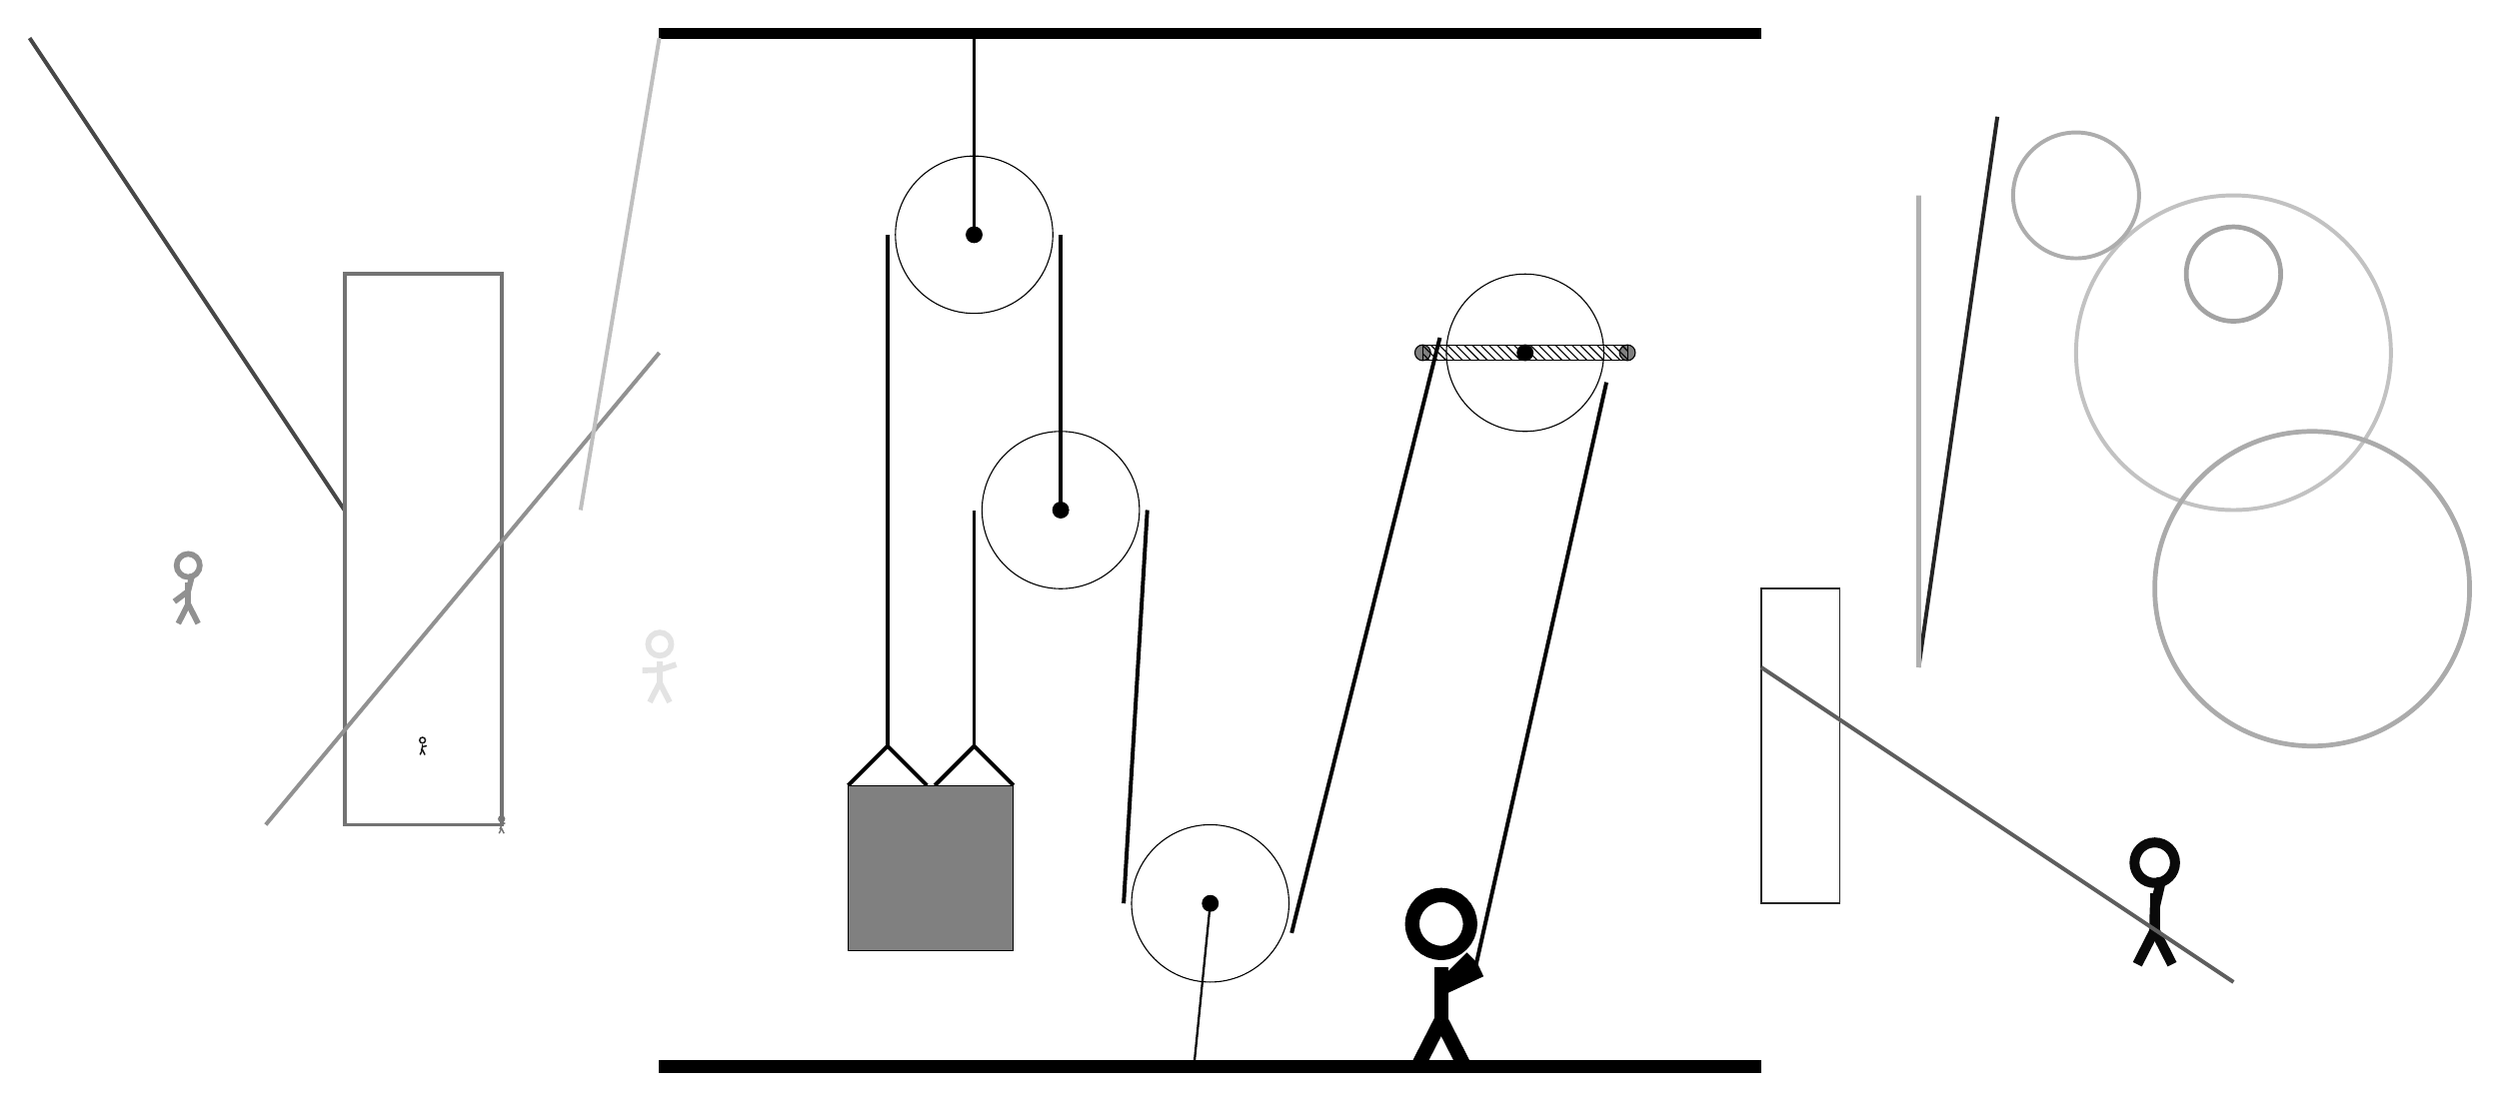
\begin{tikzpicture}
			%%%%% START %%%%%
			
			\draw[fill=black] (-2, 10) rectangle (12, 10.125);
			
			\draw (2, 7.5) circle (1);
			\draw[fill=black] (2, 7.5) circle (0.1);
			\draw[thick] (2, 7.5) -- (2, 10);
			
			\draw (3.1, 4.0) circle (1);
			\draw[fill=black] (3.1, 4.0) circle (0.1);
			
			\draw (5, -1) circle (1);
			\draw[fill=black] (5, -1) circle (0.1);
			\draw[thick] (5, -1) -- (4.8, -3);
			
			\draw (9, 6.0) circle (1);
			\draw[fill=black] (9, 6.0) circle (0.1);
			\draw[fill=black!50] (7.7, 6.0) circle (0.1);
			\draw[fill=black!50] (10.3, 6.0) circle (0.1);
			\draw[pattern=north west lines, pattern color=black] (7.7, 6.1) rectangle (10.3, 5.9);
			
			\draw[line width = 0.5mm]  (0.4, 0.5) -- (0.9, 1.0) -- (1.4, 0.5);
			\draw[line width = 0.5mm]  (1.5, 0.5) -- (2.0, 1.0) -- (2.5, 0.5);
			\draw[fill=black!50] (0.4, 0.5) rectangle (2.5, -1.6);
			
			\node[line width=0.3mm, color=black!54] at (-4, 0) {\Strichmaxerl[1][67][35]};
			
			\draw [line width=0.5mm, color=black!24](18, 6) circle (2.0);
			\draw [line width=0.5mm, color=black!32](16, 8) circle (0.8);
			\draw[line width=0.5mm, color=black!72](-6, 4) -- (-10, 10);
			
			\node[line width=0.4mm, color=black!96] at (17, -1) {\Strichmaxerl[7][89][77]};
			\draw[line width=0.5mm, color=black!86](14, 2) -- (15, 9);
			\draw[line width=0.2mm, color=black!85] (13, -1) rectangle (12, 3);
			\node[line width=0.2mm, color=black!11] at (-2, 2) {\Strichmaxerl[4][2][18]};
			\draw[line width=0.5mm, color=black!55] (-4, 7) rectangle (-6, 0);
			\draw [line width=0.6mm, color=black!33](19, 3) circle (2.0);
			\draw[line width=0.6mm, color=black!31] (14, 8) rectangle (14, 2);
			
			\draw [line width=0.6mm, color=black!36](18, 7) circle (0.6);
			\draw[line width=0.5mm, color=black!43](-7, 0) -- (-2, 6);
			
			\draw [line width=0.6mm, color=black!10](14, 4) circle (0.0);
			\draw[line width=0.5mm, color=black!63](12, 2) -- (18, -2);
			\node[line width=0.6mm, color=black!91] at (-5, 1) {\Strichmaxerl[1][75][10]};
			
			\draw[line width=0.5mm, color=black!25](-3, 4) -- (-2, 10);
			\node[line width=0.2mm, color=black!43] at (-8, 3) {\Strichmaxerl[4][37][76]};
			
			\draw[line width = 0.5mm] (0.9, 7.5) -- (0.9, 1.0);
			\centerarc[line width = 0.5mm](2, 7.5)(0:180:1.1);
			\draw[line width = 0.5mm] (3.1, 7.5) -- (3.1, 4.0);
			\draw[line width = 0.5mm] (2.0, 4.0) -- (2.0, 1.0);
			\centerarc[line width = 0.5mm](3.1, 4.0)(0:180:1.1);
			\draw[line width = 0.5mm] (4.2, 4.0) -- (3.9, -1);
			\centerarc[line width = 0.5mm](5, -1)(180:340:1.1);
			\draw[line width=0.5mm](6.0337, -1.3762) -- (7.9167, 6.191);
			\centerarc[line width = 0.5mm](9, 6.0)(-20:170:1.1);
			\draw[line width=0.5mm](10.0337, 5.6238) --  (8.35, -1.9);
			
			\node at (8, -2) {\Strichmaxerl[10][225][25]};
			
			\draw[fill=black] (-2, -3) rectangle (12, -3.15);
			
			%%%%% END %%%%%
		\end{tikzpicture}
	\end{figure}	
\end{document}